\begin{center}


\tikzset{every picture/.style={line width=0.75pt}} %set default line width to 0.75pt        

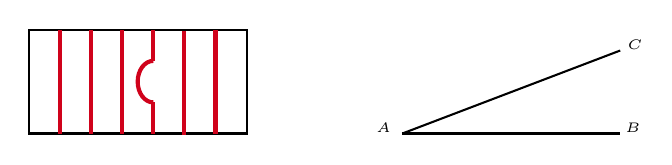
\begin{tikzpicture}[x=0.75pt,y=0.75pt,yscale=-1,xscale=1]
%uncomment if require: \path (0,300); %set diagram left start at 0, and has height of 300

%Shape: Rectangle [id:dp5450967430811406] 
\draw   (65,75) -- (170,75) -- (170,125) -- (65,125) -- cycle ;
%Straight Lines [id:da7207554445840463] 
\draw [color={rgb, 255:red, 208; green, 2; blue, 27 }  ,draw opacity=1 ][line width=1.5]    (80,75) -- (80,125) ;
%Straight Lines [id:da8856015597811548] 
\draw [color={rgb, 255:red, 208; green, 2; blue, 27 }  ,draw opacity=1 ][line width=1.5]    (95,75) -- (95,125) ;
%Straight Lines [id:da27302137833179474] 
\draw [color={rgb, 255:red, 208; green, 2; blue, 27 }  ,draw opacity=1 ][line width=1.5]    (110,75) -- (110,125) ;
%Straight Lines [id:da2045981797610763] 
\draw [color={rgb, 255:red, 208; green, 2; blue, 27 }  ,draw opacity=1 ][line width=1.5]    (125,110) -- (125,125) ;
%Straight Lines [id:da1792503962330343] 
\draw [color={rgb, 255:red, 208; green, 2; blue, 27 }  ,draw opacity=1 ][line width=1.5]    (140,75.5) -- (140,125.5) ;
%Straight Lines [id:da9645464264966506] 
\draw [color={rgb, 255:red, 208; green, 2; blue, 27 }  ,draw opacity=1 ][line width=1.5]    (155,75) -- (155,125) ;
%Straight Lines [id:da853883505351509] 
\draw [color={rgb, 255:red, 208; green, 2; blue, 27 }  ,draw opacity=1 ][line width=1.5]    (125,75) -- (125,90) ;
%Shape: Arc [id:dp6231057404985074] 
\draw  [draw opacity=0][line width=1.5]  (125,110) .. controls (120.86,110) and (117.5,105.52) .. (117.5,100) .. controls (117.5,94.48) and (120.86,90) .. (125,90) -- (125,100) -- cycle ; \draw  [color={rgb, 255:red, 208; green, 2; blue, 27 }  ,draw opacity=1 ][line width=1.5]  (125,110) .. controls (120.86,110) and (117.5,105.52) .. (117.5,100) .. controls (117.5,94.48) and (120.86,90) .. (125,90) ;  
%Straight Lines [id:da4819698726867141] 
\draw    (245,125) -- (350,125) ;
%Straight Lines [id:da2187262824312195] 
\draw    (245,125) -- (350,85) ;

% Text Node
\draw (231,118.4) node [anchor=north west][inner sep=0.75pt]  [font=\tiny]  {$A$};
% Text Node
\draw (351,118.4) node [anchor=north west][inner sep=0.75pt]  [font=\tiny]  {$B$};
% Text Node
\draw (352,78.4) node [anchor=north west][inner sep=0.75pt]  [font=\tiny]  {$C$};


\end{tikzpicture}

\end{center}